\part{Sequence of Functions}


\section{Introduction}

In previous courses, we analysed the convergence of sequences of numbers (example: $U_n = \left\{ \frac{1}{4},\frac{1}{9},\frac{1}{16},\ldots \right\} =\sum_{n=1}^{\infty} \frac{1}{n^2} $) with a series of tests. In this course we will be analysing sequences of \emph{functions} $f_n(x)$.\\
An example, is $f_n(x)=\frac{x}{x+n} =\{f_1,f_2,f_3,\ldots\}  =\left\{ \frac{x}{x+1},\frac{x}{x+2},\frac{x}{x+3},\ldots \right\}$.\\

There are 2 ways these sequences can converge: pointwise and uniformly

\begin{figure}[H]
    \centering
    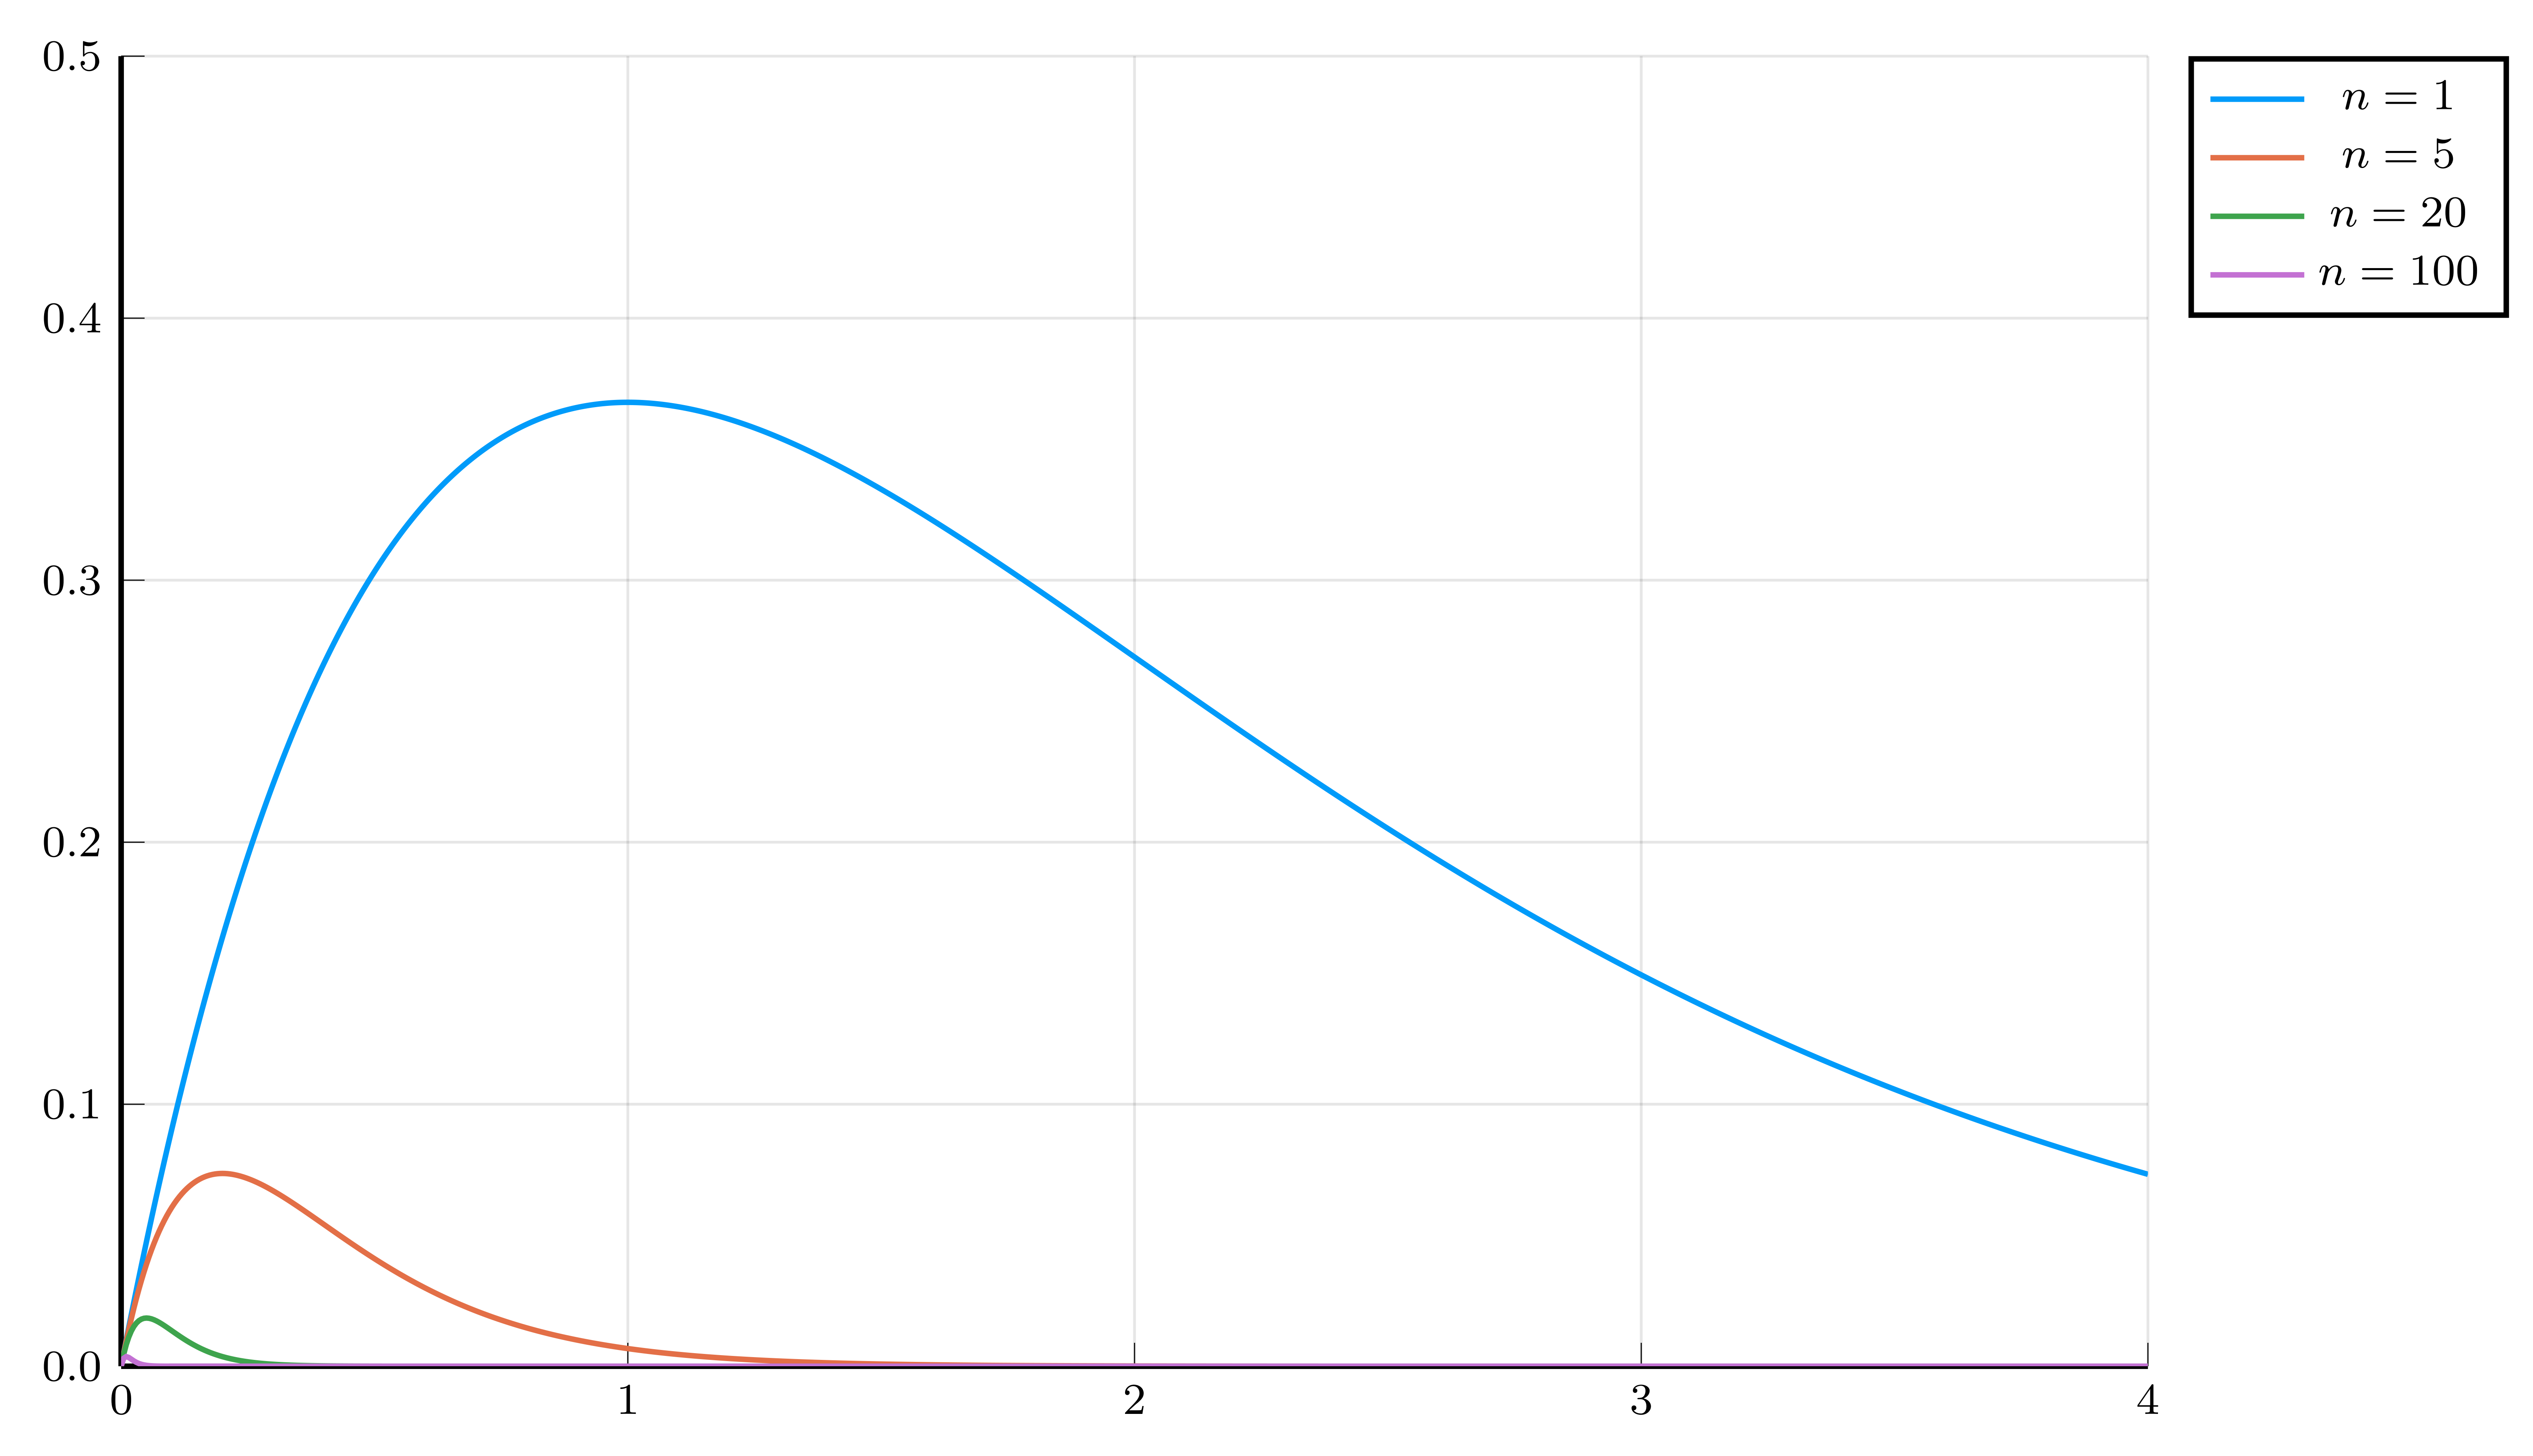
\includegraphics[width=\textwidth]{plot1.png}
    \caption*{Plot of the sequence $f_n(x)=xe^{-nx}$}
    \label{fig:plot}
\end{figure}

\section{Pointwise convergence}

This is a very natural way of proving convergence since all you have to do is fix $f_n$ to a point $x$ then the sequence just becomes an ordinary sequence of numbers, and if they all converge to a number we can define a limit function $f$ and say that they converge to $f$ pointwisely.

\begin{definition}
    We say that a sequence of functions $f_n$ where $f_n:I \to \mathbb{R},I\subset \mathbb{R}$, converges pointwise to function $f:I\to \mathbb{R}$ on the interval $I$ if:
    \[
    \forall x\in I \; \forall \epsilon >0 \; \exists n\in \mathbb{N} \; \forall n\ge \mathbb{N}: \quad \left| f_n(x)-f(x) \right|<\epsilon 
    .\] 
\end{definition}
You either prove convergence using the definition or by doing:
\begin{enumerate}
    \item Let $x=0$ then find $\lim_{n \to \infty} f_n(0)=$ some $f(x)$
    \item Then let $x\neq 0$ and again find $\lim_{n \to \infty} f_n(x)=f(x)$ 
    \item If neither of the results are unbounded $\pm \infty$ then we say $f_n(x)$ is convergent to some $f(x)$
\end{enumerate}

\begin{remark}
    if the result of step 1 is $g(x)$ and step 2 results in $h(x)$ where $g(x)\neq h(x)$ then we define the limit function:
     \[
         f(x)=\begin{cases}g(x)&x=0\\h(x)&x\in ]0,1]\end{cases}
    .\] 
\end{remark}

\section{Uniform convergence}

The idea of uniform convergence is that the sequence always approaches it's limit function as the value of $n$ increases.

\begin{definition}
    We say that a sequence of functions $f_n$ where $f_n:I \to \mathbb{R},I\subset \mathbb{R}$, converges uniformly to function $f:I\to \mathbb{R}$ on the interval $I$ if:
    \[
        \forall \epsilon>0\;\exists N\in\mathbb{N}\;\forall n\ge N\;\forall x\in I: \; \sup_{x\in I} \left| f_n(x)-f(x) \right| <\epsilon
    .\]    
\end{definition}

\begin{remark}
    We can also prove uniform convergence by proving
    \[
        \lim_{n \to \infty}\sup_{x\in I} \left| f_n(x)-f(x) \right|=0 
    .\] 
\end{remark}

There is also an easy qay to prove uniform convergence of a function by
\begin{enumerate}
    \item Prove that the sequence of fucntions $f_n(x)$ is pointwise convergent to a function $f(x)$ \mn{if the function $f(x)$ is continuous at a point piecewise the the sequence doesn't uniformly}
        \item Define a function $g(x)=|f_n(x)-f(x)|$ and find the maxima of that function at a point $x_0$ (usually by doing $\dv*{g}{x} =0$)
            \item If $\lim_{n \to \infty}g(x_0)=0 $ then the sequence converges uniformly to $f(x)$
\end{enumerate}



